\documentclass[12pt,a4paper]{article}

\usepackage[utf8]{inputenc}
\usepackage{geometry}
\usepackage{indentfirst}
\usepackage{graphicx}
\usepackage{longtable}
\usepackage{array}

\geometry{margin=2.5cm}
\renewcommand{\arraystretch}{1.2}
\setlength{\parindent}{1.25cm}
\linespread{1.3}

\title{\textbf{Relatório Final do Projeto}\\Agentic Customer Intelligence}
\author{Gabriel Cravalho Domingos da Conceição}
\date{Maio de 2026}

\begin{document}

\maketitle

\begin{abstract}
Este documento apresenta a formulação do problema, a solução técnica desenvolvida, os métodos de aprendizado de máquina utilizados, a camada agentic baseada em personas, a arquitetura da aplicação, os resultados obtidos e as principais avaliações realizadas. O projeto integra segmentação não supervisionada de consumidores, geração de personas sintéticas, recuperação de contexto com \textit{retrieval augmented generation} (RAG), API em FastAPI e interface web em React para apoiar exploração de hipóteses comerciais.
\end{abstract}

\section{Padrão de Formatação}

Este documento segue diretrizes formais alinhadas ao padrão ABNT para trabalhos técnicos: papel A4, fonte serifada do tipo Times, corpo 12, margens de 2,5 cm, espaçamento de 1,5 e recuo de parágrafo de 1,25 cm.

\section{Formulação do Problema}

O problema abordado consiste em transformar uma base de consumidores em uma ferramenta de inteligência de mercado capaz de responder perguntas de negócio sobre preço, promoções, canais, preferência de marca e frequência de compra. O desafio não era apenas clusterizar clientes, mas tornar os segmentos acionáveis para usuários de negócio por meio de uma interface conversacional.

Foram definidos três objetivos principais:

\begin{enumerate}
  \item Identificar segmentos de consumidores com base em padrões comportamentais e transacionais.
  \item Traduzir os segmentos em personas sintéticas com linguagem natural e sinais comportamentais distintos.
  \item Disponibilizar uma experiência de chat na qual stakeholders possam comparar respostas de segmentos ou conversar com uma persona específica.
\end{enumerate}

A solução deveria preservar rastreabilidade e coerência: as respostas das personas deveriam permanecer ancoradas no perfil estatístico dos clusters, evitando que o modelo de linguagem inventasse características não observadas.

\section{Visão Geral da Solução}

A solução final foi organizada em quatro camadas:

\begin{itemize}
  \item \textbf{Pipeline de Machine Learning}: leitura, validação, preparação de atributos, clusterização e geração de perfis.
  \item \textbf{Camada de Personas}: transformação dos clusters em agentes sintéticos com regras de resposta e sinais comportamentais.
  \item \textbf{Backend RAG}: API em FastAPI, persistência de conversas, recuperação de documentos por persona e integração com LLM local compatível com OpenAI.
  \item \textbf{Frontend}: aplicação React/Vite para iniciar conversas coletivas ou individuais e comparar respostas por segmento.
\end{itemize}

O fluxo lógico é:

\begin{center}
\texttt{dados sintéticos -> clustering -> perfis -> personas -> RAG -> API -> interface web}
\end{center}

\section{Métodos de Machine Learning}

\subsection{Preparação dos Dados}

A base utilizada foi \texttt{data/dados\_sinteticos.csv}. O pipeline de ML executa:

\begin{itemize}
  \item validação de esquema e qualidade mínima dos dados;
  \item engenharia de variáveis derivadas, incluindo idade e faixa etária;
  \item codificação de variáveis categóricas de alta cardinalidade por frequência;
  \item codificação \textit{one-hot} para variáveis categóricas de baixa cardinalidade;
  \item normalização de variáveis numéricas;
  \item avaliação de diferentes valores de $k$ para KMeans;
  \item exportação de perfis interpretáveis para uso na camada agentic.
\end{itemize}

\subsection{Algoritmo Selecionado}

O método principal escolhido foi KMeans, implementado com \texttt{scikit-learn}. A escolha foi motivada por quatro fatores:

\begin{enumerate}
  \item simplicidade operacional;
  \item facilidade de explicar os segmentos para stakeholders;
  \item compatibilidade com atributos transformados e normalizados;
  \item integração direta com métricas internas de clusterização.
\end{enumerate}

Foram avaliados valores de $k$ entre 2 e 8. Embora $k=2$ tenha apresentado maior \textit{silhouette} em parte das avaliações, $k=3$ foi selecionado por oferecer melhor equilíbrio entre qualidade métrica e interpretabilidade de negócio.

\subsection{Métricas Avaliadas}

As principais métricas internas foram:

\begin{itemize}
  \item \textit{Silhouette Score}: mede separação e coesão dos clusters;
  \item \textit{Davies-Bouldin Score}: menor valor indica melhor separação relativa;
  \item \textit{Calinski-Harabasz Score}: maior valor indica melhor dispersão entre grupos em relação à dispersão interna;
  \item inércia e curva de \textit{elbow}.
\end{itemize}

\begin{longtable}{|c|r|r|r|r|}
\hline
\textbf{k} & \textbf{Inércia} & \textbf{Silhouette} & \textbf{Davies-Bouldin} & \textbf{Calinski-Harabasz} \\
\hline
2 & 22537.23 & 0.0896 & 3.0900 & 304.13 \\
3 & 21112.35 & 0.0805 & 2.7574 & 263.41 \\
4 & 20019.61 & 0.0781 & 2.5311 & 239.64 \\
5 & 19135.89 & 0.0761 & 2.3746 & 222.55 \\
6 & 18411.26 & 0.0770 & 2.2500 & 208.55 \\
7 & 17881.80 & 0.0728 & 2.3582 & 193.65 \\
8 & 17499.86 & 0.0709 & 2.3041 & 178.88 \\
\hline
\end{longtable}

\begin{figure}[htbp]
\centering
\includegraphics[width=0.72\textwidth]{../ml-clustering/outputs/figures/elbow_method.png}
\caption{Curva de \textit{elbow} para seleção de $k$ no KMeans}
\end{figure}

\begin{figure}[htbp]
\centering
\includegraphics[width=0.72\textwidth]{../ml-clustering/outputs/figures/silhouette_scores.png}
\caption{Evolução do \textit{Silhouette Score} por número de clusters}
\end{figure}

\section{Segmentos Encontrados}

O resultado final produziu três clusters.

\begin{longtable}{|p{4.1cm}|r|r|r|p{5.0cm}|}
\hline
\textbf{Segmento} & \textbf{Share} & \textbf{Idade média} & \textbf{Ticket médio} & \textbf{Principais sinais} \\
\hline
Consumidores Maduros do Norte com Pagamento Digital & 35.2\% & 58.2 & R\$ 120.45 & Região Norte, loja física, bebidas, compras semanais, carteira digital, faixa 55+. \\
\hline
Jovens Adultos Recorrentes do Sudeste & 34.2\% & 30.0 & R\$ 123.36 & Sudeste, loja física, bebidas, compras semanais, crédito, faixa 25--34. \\
\hline
Consumidores Mainstream Recorrentes do Sudeste & 30.6\% & 45.4 & R\$ 121.66 & Sudeste, loja física, bebidas, compras semanais, crédito, comportamento mais próximo da média. \\
\hline
\end{longtable}

Os segmentos foram utilizados não apenas como rótulos, mas como fonte primária de comportamento para as personas. Cada persona possui sinais de diferenciação e limites explícitos para evitar respostas genéricas.

\begin{figure}[htbp]
\centering
\includegraphics[width=0.9\textwidth]{../ml-clustering/outputs/figures/clusters_pca_2d.png}
\caption{Visualização bidimensional dos clusters (projeção PCA)}
\end{figure}

\begin{figure}[htbp]
\centering
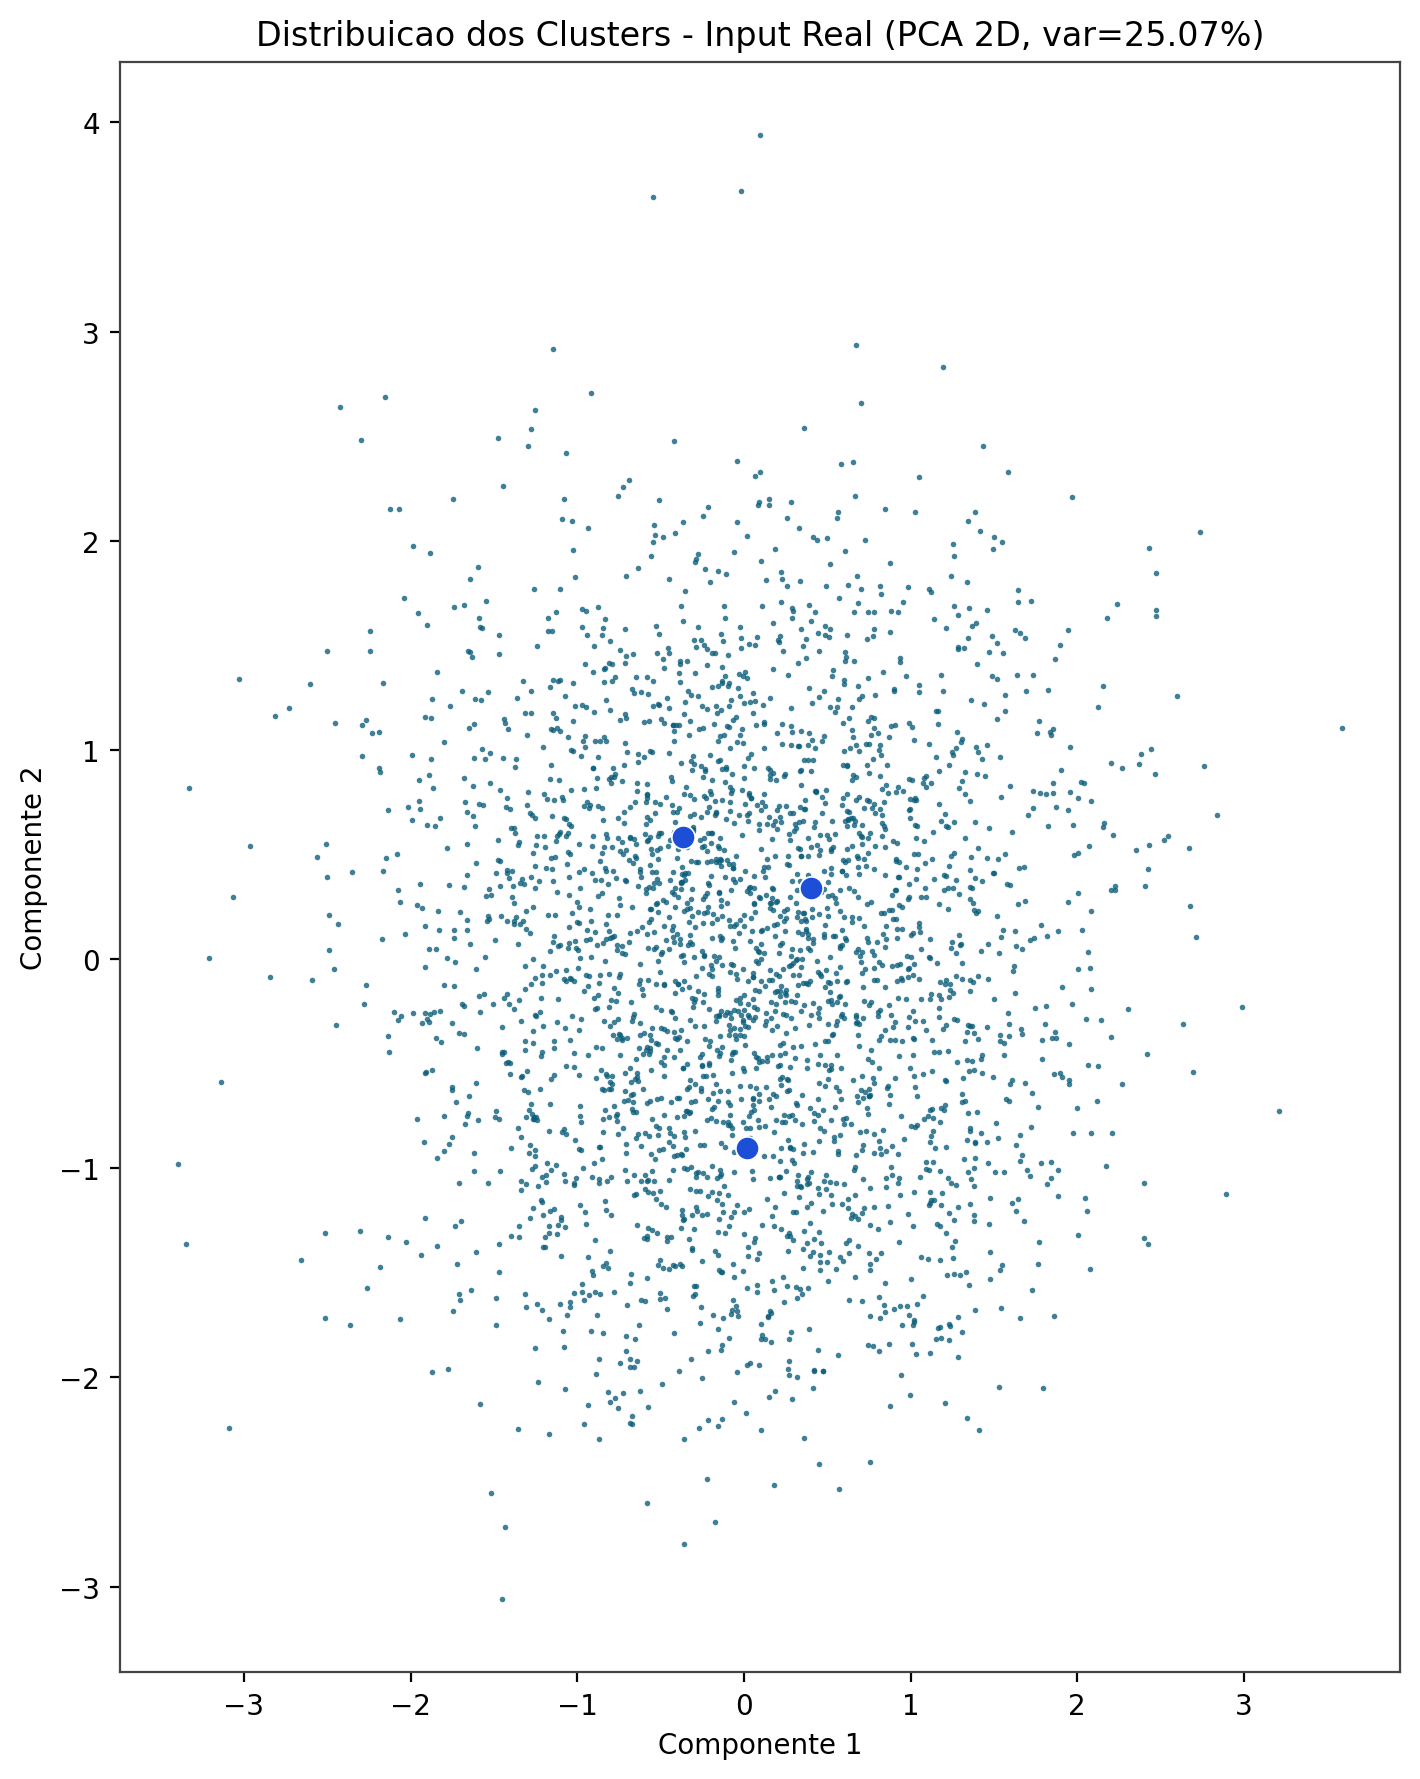
\includegraphics[width=0.8\textwidth]{cluster_input_distribution_real_styled.png}
\caption{Distribuição dos principais sinais de entrada por cluster}
\end{figure}

\section{Camada Agentic e RAG}

\subsection{Motivação}

Uma segmentação tradicional gera tabelas e gráficos, mas exige interpretação constante do usuário. A camada agentic foi adicionada para permitir perguntas em linguagem natural e simulação qualitativa de respostas por segmento.

\subsection{Fontes de Informação}

A arquitetura RAG utiliza duas classes de fonte:

\begin{itemize}
  \item \textbf{Fonte primária}: perfis estatísticos exportados em \texttt{cluster\_profiles.json}.
  \item \textbf{Fonte secundária}: base de conhecimento Markdown em \texttt{agentic-personas/knowledge\_base}, com documentos compartilhados e documentos específicos por persona.
\end{itemize}

A recuperação é persona-aware: ao responder como a Persona 0, o sistema recupera documentos da própria Persona 0 e documentos compartilhados, mas não recupera documentos das Personas 1 ou 2. Isso reduz contaminação entre perfis.

\subsection{Validação de Qualidade de Respostas}

Foi implementado um validador final para respostas, com foco em:

\begin{itemize}
  \item naturalidade em português brasileiro;
  \item concisão;
  \item aderência ao cluster;
  \item ancoragem no RAG;
  \item diferenciação entre personas;
  \item remoção de fragmentos malformados e frases genéricas.
\end{itemize}

Quando uma resposta falha na validação, o sistema aciona reescrita ou fallback direcionado por pergunta e persona. Esse mecanismo foi importante para perguntas críticas de marketing, como aumento de preço, combo promocional e escolha recorrente de marca.

\section{Tecnologias Escolhidas}

\begin{longtable}{|p{4cm}|p{10cm}|}
\hline
\textbf{Componente} & \textbf{Tecnologia e justificativa} \\
\hline
Gerenciamento Python & \texttt{uv}, por velocidade, reprodutibilidade e simplicidade para ambientes locais. \\
\hline
Machine Learning & \texttt{pandas}, \texttt{scikit-learn}, \texttt{matplotlib} e \texttt{seaborn}, por maturidade e clareza em pipelines tabulares. \\
\hline
Backend & FastAPI, por tipagem, documentação automática e facilidade para endpoints síncronos e streaming. \\
\hline
RAG & PostgreSQL com pgvector, por permitir busca vetorial em infraestrutura SQL conhecida. \\
\hline
Persistência de conversas & MongoDB, por flexibilidade para histórico de mensagens e metadados variáveis. \\
\hline
LLM local & API local compatível com OpenAI, permitindo alternar modelos e embeddings sem acoplar o backend a um provedor específico. \\
\hline
Frontend & React, TypeScript e Vite, por produtividade e boa experiência de desenvolvimento para interfaces interativas. \\
\hline
Infraestrutura local & Docker Compose para MongoDB e PostgreSQL/pgvector. \\
\hline
\end{longtable}

\section{Interface e Experiência do Usuário}

A interface final permite:

\begin{itemize}
  \item iniciar chat coletivo com as três personas;
  \item iniciar chat individual a partir de cards visuais de cada persona;
  \item selecionar personas ativas na barra lateral;
  \item limpar ou excluir conversas;
  \item gerar novamente ou editar a última pergunta;
  \item persistir histórico em MongoDB;
  \item exibir título curto de conversa baseado na primeira pergunta;
  \item mostrar avatar da persona nas respostas.
\end{itemize}

Os cards da tela inicial foram montados como componentes HTML/CSS usando imagens das personas como fotografia principal, evitando depender de imagens de cards inteiros.

\section{Resultados e Avaliações}

\subsection{Resultados de Segmentação}

A segmentação identificou três grupos com diferenças acionáveis em idade, região, pagamento e comportamento de compra. A Persona 2 foi reconhecida como mais próxima da média da base, o que foi tratado explicitamente nas respostas por meio de linguagem mais cautelosa e foco em previsibilidade.

\subsection{Resultados da Bateria de Respostas}

A bateria final de qualidade para as personas foi executada em 15 perguntas de marketing e comportamento. O resultado final foi:

\begin{itemize}
  \item \textbf{overall\_score}: 5.0;
  \item \textbf{target\_score}: 4.0;
  \item \textbf{failed\_question\_count}: 0;
  \item \textbf{passed}: verdadeiro;
  \item \textbf{differentiation\_score}: 5.0 em todas as perguntas avaliadas.
\end{itemize}

As perguntas cobriram troca de marca, aumento de preço, promoções, primeira compra de nova marca, benefícios, canal digital, comunicação, frequência de compra, combos promocionais, abandono de marca, momento de impacto, confiabilidade da comunicação, personalização e recorrência de escolha.

\subsection{Comparações}

Foram comparadas variações da segmentação e iterações da camada de respostas. Em ML, a decisão por $k=3$ privilegiou a combinação entre métrica e interpretabilidade. Na camada agentic, versões com respostas mais curtas tiveram pior diferenciação em perguntas importantes; a versão final restaurou sinais específicos por persona e manteve validação formal.

\section{Limitações}

As principais limitações são:

\begin{itemize}
  \item a base de dados é sintética;
  \item métricas internas de clusterização apresentaram valores modestos de separação;
  \item o desempenho qualitativo das personas depende da qualidade dos prompts, dos fallbacks e do modelo local;
  \item a interpretação dos clusters deve ser validada com dados reais e feedback de negócio antes de uso produtivo.
\end{itemize}

\section{Conclusão}

O projeto entregou uma solução integrada de inteligência de clientes, combinando segmentação não supervisionada, geração de personas sintéticas, RAG, persistência de conversas e interface conversacional. A solução permite transformar uma análise estática de clusters em uma ferramenta interativa para explorar decisões de marketing e comportamento de consumidores.

O resultado final é adequado para demonstração técnica e de negócio, com avaliação automatizada de qualidade das respostas e experiência de usuário orientada a comparação entre segmentos.

\end{document}
